\documentclass[aspectratio=169]{beamer}
\usepackage[UTF8]{ctex}  % 支持中文
\usepackage{graphicx}    % 图片支持
\usepackage{booktabs}    % 表格美化
\usepackage{hyperref}    % 超链接
\usepackage{amsmath}     % 数学公式
\usepackage{multirow}    % 表格合并单元格
\usepackage{xcolor}      % 颜色支持
\usepackage{wrapfig}  
% ... 已有代码 ...

% beamer主题设置
\usetheme{Madrid}        % 使用Madrid主题,该主题包含标题栏、导航条和页脚等元素
\usecolortheme{spruce}    % 颜色主题,此处指定Spruce主题
\usefonttheme{professionalfonts} % 使用专业字体主题,让文档使用默认或用户自定义字体
\setbeamertemplate{navigation symbols}{}  % 移除幻灯片右下角默认显示的导航按钮(如前进、后退、缩放等)
\setbeamertemplate{footline}[frame number]  % 在幻灯片底部添加页码

% 导航条设置
\useoutertheme[subsection=false]{miniframes} % 使用miniframes外部主题,且不显示子节导航
\makeatletter % 临时改变对@字符的解释,允许使用包含@的内部命令
\setbeamertemplate{headline}{%
  % 创建一个高度为2.25ex、深度为1ex的颜色盒子,使用section in head/foot颜色主题
  \begin{beamercolorbox}[ht=3ex,dp=1ex]{section in head/foot}
    \insertnavigation{\paperwidth} % 在颜色盒子中插入宽度为纸张宽度的导航条
  \end{beamercolorbox}%
}
\makeatother % 恢复对@字符的默认解释

% 自定义frametitle模板,添加垂直间距
\makeatletter % 临时改变对@字符的解释,允许使用包含@的内部命令
\setbeamertemplate{frametitle}{%
  % 检查标题背景颜色是否为空,若不为空则禁止插入额外的行距
  \ifbeamercolorempty[bg]{frametitle}{}{\nointerlineskip}%
  \@tempdima=\textwidth% 临时变量存储文本宽度
  \advance\@tempdima by\beamer@leftmargin% 加上左侧边距
  \advance\@tempdima by\beamer@rightmargin% 加上右侧边距
  % 创建一个颜色盒子,内边距0.3cm,左对齐,宽度为之前计算的值,使用frametitle颜色主题
  \begin{beamercolorbox}[sep=0.3cm,left,wd=\the\@tempdima]{frametitle}
    \usebeamerfont{frametitle}% 使用Beamer定义的标题字体
    \vbox{}\vskip-1ex% 创建垂直盒子并向上移动1ex
    % 根据条件调用内部命令,控制标题的对齐方式
    \if@tempswa\else\csname beamer@fteleft\endcsname\fi%
    \strut\insertframetitle\strut\par% 插入幻灯片标题,并添加垂直间距保证高度一致
    {%
      % 检查是否有副标题,若有则插入副标题
      \ifx\insertframesubtitle\@empty%
      \else%
      {\usebeamerfont{framesubtitle}\usebeamercolor[fg]{framesubtitle}\insertframesubtitle\strut\par}%
      \fi
    }%
    \vskip-1ex% 向上移动1ex
    % 根据条件调整垂直间距
    \if@tempswa\else\vskip-.3cm\fi%
    \vspace{1em} % 在标题内容之后添加1em的垂直间距,可按需调整该值
  \end{beamercolorbox}%
}
\makeatother % 恢复对@字符的默认解释

% ... 已有代码 ...



% 标题信息
\title{新能源在分布式能源的应用情况}

\author{演讲人,组员,组员 \\报告人\textbf{:演讲人}}
\institute{东莞理工学院}
\date{\today}

\begin{document}

% 标题页
\begin{frame}
  \titlepage
\end{frame}

% 目录页
\begin{frame}{报告大纲}
  \tableofcontents
\end{frame}

% 第一章:引言
\section{引言}

\begin{frame}{背景与意义}
  \begin{itemize}
    \item \textbf{能源转型的关键时期}
      \begin{itemize}
        \item 中国碳达峰、碳中和政策的推进\cite{Zhou2022}
        \item 能源系统面临的挑战:安全性、经济性、环保性
      \end{itemize}
    \item \textbf{分布式能源系统概念}
      \begin{itemize}
        \item 定义:靠近负荷侧、小型模块化的能源生产和供应系统
        \item 特点:灵活部署、就近消纳、减少输配环节损耗
      \end{itemize}
    \item \textbf{新能源与分布式能源的融合意义}
      \begin{itemize}
        \item 提升能源利用效率,降低碳排放
        \item 促进能源消费方式变革,构建清洁低碳能源体系\cite{Li2021}
      \end{itemize}
  \end{itemize}
\end{frame}

\begin{frame}{研究问题与目标}
  \begin{itemize}
    \item \textbf{研究问题}
      \begin{itemize}
        \item 如何有效整合各类新能源技术到分布式能源系统?
        \item 不同新能源技术在分布式应用中的适应性如何?
        \item 我国分布式新能源系统发展面临的关键问题与对策?
      \end{itemize}
    \item \textbf{报告目标}
      \begin{itemize}
        \item 分析新能源技术在分布式能源系统中的应用特点
        \item 介绍国内外代表性案例和最新进展
        \item 探讨未来发展趋势和技术路线\cite{Wang2023}
      \end{itemize}
  \end{itemize}
\end{frame}

% 第二章:新能源类型与优越性分析
\section{新能源类型与优越性分析}

\begin{frame}{新能源技术分类}
  \begin{table}
    \centering
    \small
    \begin{tabular}{llcc}
      \toprule
      \textbf{能源类型} & \textbf{主要技术} & \textbf{资源特性} & \textbf{适用场景} \\
      \midrule
      太阳能 & 光伏发电、光热利用 & 间歇性、可预测 & 城市建筑、农村地区 \\
      风能 & 风力发电(小型、微型) & 间歇性、季节性 & 沿海、高地、开阔区域 \\
      生物质能 & 生物质气化、沼气利用 & 稳定性、可调度 & 农村、畜牧业区域 \\
      地热能 & 地热供暖、地源热泵 & 稳定性、持续性 & 建筑供暖制冷 \\
      小水电 & 微型水力发电 & 季节性、可调度 & 山区、河流地区 \\
      海洋能 & 潮汐能、波浪能 & 周期性、可预测 & 沿海地区 \\
      氢能 & 燃料电池、储能系统 & 灵活性、可调度 & 交通、工业、建筑 \\
      \bottomrule
    \end{tabular}
    \caption{分布式能源系统中的主要新能源类型\cite{Zhang2022}}
  \end{table}
\end{frame}

\begin{frame}{各类新能源优越性分析}
  \begin{table}
    \centering
    \small
    \begin{tabular}{lccccc}
      \toprule
      \textbf{能源类型} & \textbf{资源丰富度} & \textbf{技术成熟度} & \textbf{经济性} & \textbf{环保性} & \textbf{灵活性} \\
      \midrule
      太阳能 & \textcolor{green!70!black}{高} & \textcolor{green!70!black}{高} & \textcolor{green!70!black}{高} & \textcolor{green!70!black}{极高} & \textcolor{yellow!70!black}{中} \\
      风能 & \textcolor{green!70!black}{高} & \textcolor{green!70!black}{高} & \textcolor{green!70!black}{高} & \textcolor{green!70!black}{极高} & \textcolor{red!70!black}{低} \\
      生物质能 & \textcolor{yellow!70!black}{中} & \textcolor{yellow!70!black}{中} & \textcolor{yellow!70!black}{中} & \textcolor{yellow!70!black}{中} & \textcolor{green!70!black}{高} \\
      地热能 & \textcolor{red!70!black}{低} & \textcolor{yellow!70!black}{中} & \textcolor{yellow!70!black}{中} & \textcolor{green!70!black}{高} & \textcolor{green!70!black}{高} \\
      
      小水电 & \textcolor{yellow!70!black}{中} & \textcolor{green!70!black}{高} & \textcolor{green!70!black}{高} & \textcolor{green!70!black}{高} & \textcolor{yellow!70!black}{中} \\
      海洋能 & \textcolor{yellow!70!black}{中} & \textcolor{red!70!black}{低} & \textcolor{red!70!black}{低} & \textcolor{green!70!black}{高} & \textcolor{red!70!black}{低} \\
      氢能 & \textcolor{green!70!black}{高} & \textcolor{yellow!70!black}{中} & \textcolor{red!70!black}{低} & \textcolor{green!70!black}{极高} & \textcolor{green!70!black}{极高} \\
      
      \bottomrule
    \end{tabular}
    \caption{各类新能源在分布式应用中的优越性对比\cite{Chen2024}}
  \end{table}
\end{frame}



\begin{frame}{光伏发电系统技术特点与优越性}
  \begin{columns}
    % 左侧文字部分,占 0.6 宽度
    \column{0.6\textwidth}
    \begin{itemize}
      \item \textbf{技术优势}
        \begin{itemize}
          \item 零污染、零排放,环保性极高
          \item 模块化设计,规模灵活可调
          \item 维护简单,无运动部件
          \item 经济性持续提升(LCOE从2010年的1.83元/kWh降至2023年的0.3元/kWh)\cite{Wang2023}
        \end{itemize}
      \item \textbf{应用情境}
        \begin{itemize}
          \item 建筑屋顶、幕墙一体化(BIPV)
          \item 农光互补、渔光互补模式
          \item 微电网核心能源
        \end{itemize}
    \end{itemize}
    % 右侧图片部分,占 0.4 宽度
    \column{0.4\textwidth}
    \begin{figure}
      \centering
      \caption{光伏技术成本下降趋势}
      % 实际使用时替换为真实图片
      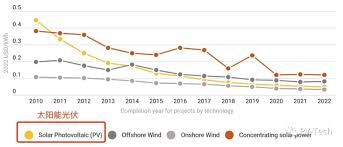
\includegraphics[width=\textwidth]{fig/光伏价格趋势.jpg}
    \end{figure}
  \end{columns}
\end{frame}

\begin{frame}{风能与生物质能的应用特点}
  \begin{columns}
    % 左侧分布式风能系统部分,占 0.5 宽度
    \column{0.5\textwidth}
    \textbf{分布式风能系统}
    \begin{itemize}
      \item 小型风机(<100kW)适用于分散区域
      \item 优势:设备成本下降、简化并网流程
      \item 挑战:风资源不确定性、噪声干扰
      \item 适用场景:农村、海岛、风资源丰富区域
      \item 技术进步:垂直轴、低风速风机技术\cite{Li2023}
    \end{itemize}
    % 右侧生物质能系统部分,占 0.5 宽度
    \column{0.5\textwidth}
    \textbf{生物质能系统}
    \begin{itemize}
      \item 形式:沼气池、气化炉、直燃锅炉等
      \item 优势:资源可再生、可调度性强
      \item 技术路线:热电联产、多联产系统
      \item 应用领域:农村能源、工业园区
      \item 发展趋势:提高气化效率、降低排放\cite{Zhang2021}
    \end{itemize}
  \end{columns}
\end{frame}

% 第三章:案例研究
\section{新能源分布式应用案例研究}

\begin{frame}{光伏分布式发电系统案例}
  \begin{columns}
    % 左侧文字部分,占 0.7 宽度
    \column{0.7\textwidth}
    \textbf{案例:江苏省常州市金坛区"光伏小镇"项目}
    \begin{itemize}
      \item \textbf{项目概况}:
        \begin{itemize}
          \item 覆盖面积:约12平方公里,2000多户居民
          \item 装机规模:户用光伏15MW,集中式10MW
          \item 投资规模:约2.5亿元,2019年开始建设\cite{Sun2022}
        \end{itemize}
      \item \textbf{技术特点}:
        \begin{itemize}
          \item "自发自用、余电上网"模式
          \item 智能微电网技术,配备储能装置
          \item 采用"光伏+5G+物联网"智慧能源管理系统
        \end{itemize}
      \item \textbf{项目成效}:
        \begin{itemize}
          \item 年均发电量约3000万kWh,减排$CO_2$约2.8万吨
          \item 居民年均增收3000-5000元,创建清洁能源示范区
        \end{itemize}
    \end{itemize}
    % 右侧图片部分,占 0.3 宽度
    \column{0.3\textwidth}
    \begin{figure}
      \centering
      \caption{常州市金坛区发展和改革局报告}
      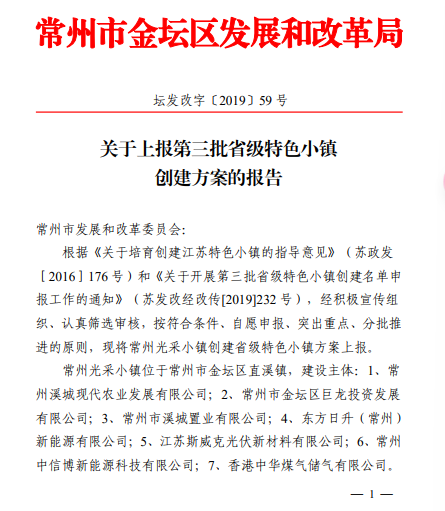
\includegraphics[width=\textwidth]{fig/光伏小镇.png}
    \end{figure}
  \end{columns}
\end{frame}

\begin{frame}{风能分布式应用案例}
  \begin{columns}
    % 左侧文字部分,占 0.7 宽度
    \column{0.7\textwidth}
    \textbf{案例:浙江舟山群岛智慧能源微网系统}
    \begin{itemize}
      \item \textbf{项目背景}:
        \begin{itemize}
          \item 地点:舟山群岛嵊山岛
          \item 岛屿面积:约15.6平方公里,常住人口约8000人
          \item 项目启动:2018年,国家能源局海岛智慧能源示范项目\cite{Chen2021}
        \end{itemize}
      \item \textbf{系统构成}:
        \begin{itemize}
          \item 分布式风电:10台100kW小型风机,总装机1MW
          \item 配套系统:3MW光伏,2MWh储能系统
          \item 智慧控制:能源管理系统与需求侧响应
        \end{itemize}
      \item \textbf{项目亮点}:
        \begin{itemize}
          \item 实现了岛屿电力"自发自用、余电上网"
          \item 年均风电发电量约235万kWh,减少柴油机组使用
          \item 降低用电成本约30\%,提高供电可靠性达99.9\%
        \end{itemize}
    \end{itemize}
    % 右侧图片部分,占 0.3 宽度
    \column{0.3\textwidth}
    \begin{figure}
      \centering
      \caption{全国首个自愈式海岛智慧微电网投运——《中国能源报》}
      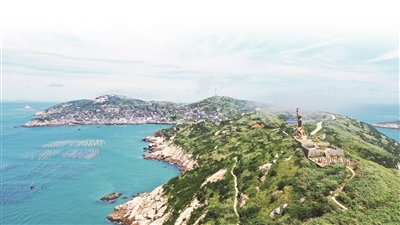
\includegraphics[width=\textwidth]{fig/全国首个自愈式海岛智慧微电网投运.jpg}
    \end{figure}
  \end{columns}
\end{frame}

\begin{frame}{生物质能应用案例}
  \begin{columns}
    % 左侧文字部分,占 0.6 宽度
    \column{0.6\textwidth}
    \textbf{案例:浙能龙泉生物质发电项目}
    \begin{itemize}
      \item 原料来源:以木屑、竹屑、废弃菌菇棒等农林废弃物为主,年处理量约 25 万吨,消纳当地及周边地区林产品加工废料和食用菌废菌棒超 20 万吨 / 年。
      \item 运行模式:采用生物质直接燃烧发电技术,融合光伏发电形成 “自发自用、余量上网” 模式;通过抽汽供热管路改造,为周边小微工业园区提供工业蒸汽,推动区域集中供热集约化。
      \item 经济效益:截至 2023 年,累计发电 14.79 亿千瓦时,节省标煤 71.01 万吨,减少二氧化碳排放 194.71 万吨;年均带动农民增收 7500 万元,九年累计惠农超 6.07 亿元。
    \end{itemize}
    \column{0.4\textwidth}
    \begin{figure}
      \centering
      \caption{浙能龙泉生物质发电项目——政府报告}
      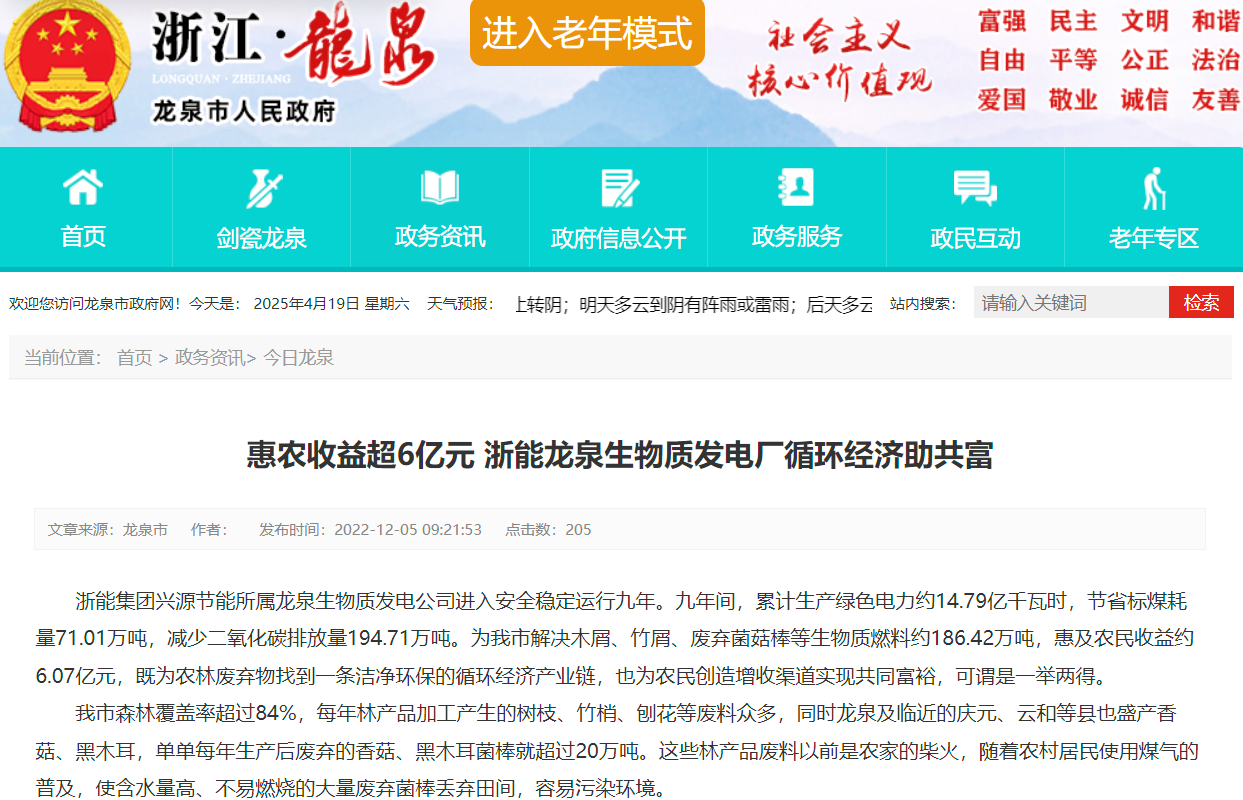
\includegraphics[width=\textwidth]{fig/浙能龙泉生物质发电项目.png}
    \end{figure}
  \end{columns}
\end{frame}

\begin{frame}{地热能应用案例}
  \begin{columns}
    \column{0.6\textwidth}
    \textbf{案例:西安浐灞生态区地热能供暖项目}
    \begin{itemize}
      \item 项目规模:覆盖面积120万平方米,服务约2万户居民
      \item 技术路线:浅层地热能与地源热泵系统结合
      \item 环保效益:替代传统燃煤锅炉,年减少碳排放约4.2万吨
      \item 经济性:较传统供暖节约运行成本约2\%\cite{Yang2023}
    \end{itemize}
    % 右侧图片部分,占 0.4 宽度
    \column{0.4\textwidth}
    \begin{figure}
      \centering
      \caption{西安浐灞生态区获联合国环境署点赞—— 陕西省地热协会}
      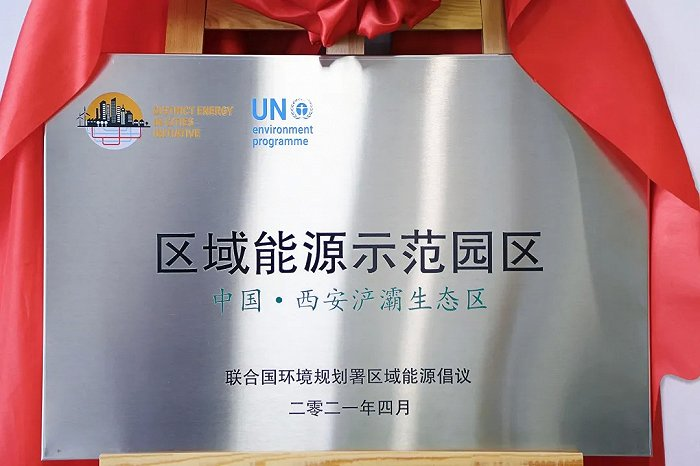
\includegraphics[width=\textwidth]{fig/西安浐灞生态区.jpg}
    \end{figure}
  \end{columns}
\end{frame}

\begin{frame}{氢能与综合能源系统案例}
  \begin{columns}
    % 左侧文字部分,占 0.6 宽度
    \column{0.6\textwidth}
    \textbf{案例:张家口可再生能源示范区氢能应用}
    \begin{itemize}
      \item \textbf{项目概况}:
        \begin{itemize}
          \item 地点:河北张家口市崇礼区
          \item 背景:2022年冬奥会氢能示范应用
          \item 规模:风电制氢装置4MW,储氢规模200kg/天\cite{Wu2023}
        \end{itemize}
      \item \textbf{系统架构}:
        \begin{itemize}
          \item "风光氢储一体化"分布式能源系统
          \item 氢能公交、物流车队,固定式加氢站
          \item 燃料电池分布式发电系统(为冬奥场馆供电)
        \end{itemize}
      \item \textbf{创新点}:
        \begin{itemize}
          \item 首个大规模可再生能源制氢示范应用
          \item 解决了弃风弃光问题,提高可再生能源利用率
          \item 建立了完整的氢能产业链闭环
        \end{itemize}
    \end{itemize}
    % 右侧图片部分,占 0.4 宽度
    \column{0.4\textwidth}
    \begin{figure}
      \centering
      \caption{张家口:加快推进可再生能源示范区跨越式发展——人民日报}
      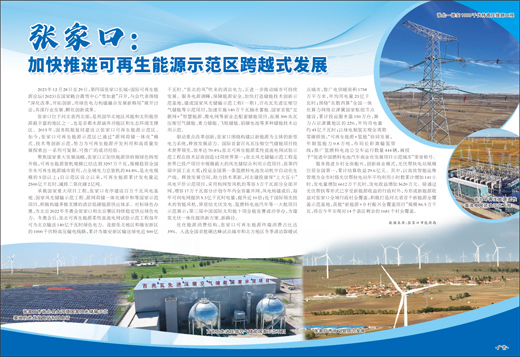
\includegraphics[width=\textwidth]{fig/张家口:加快推进可再生能源示范区跨越式发展.jpg}
    \end{figure}
  \end{columns}
\end{frame}

% ... 已有代码 ...
% 第四章:发展趋势与前景
\section{发展趋势与前景展望}

\begin{frame}{新能源分布式系统发展趋势}
  \begin{itemize}
    \item \textbf{技术融合与集成创新}
      \begin{itemize}
        \item "源-网-荷-储"一体化智慧能源系统
        \item 多能互补系统优化配置与协调控制
        \item 数字化、智能化技术深度应用\cite{Li2024}
      \end{itemize}
    \item \textbf{商业模式创新}
      \begin{itemize}
        \item 虚拟电厂、能源区块链、能源共享经济
        \item 分布式发电市场化交易机制
        \item "能源即服务"新型商业模式
      \end{itemize}
    \item \textbf{政策机制完善}
      \begin{itemize}
        \item 分布式发电上网电价机制改革
        \item 能源互联网标准体系建设
        \item 碳交易市场对分布式能源的激励机制\cite{Wang2024}
      \end{itemize}
  \end{itemize}
\end{frame}

\begin{frame}{结论与展望}
  \begin{itemize}
    \item \textbf{研究结论}
      \begin{itemize}
        \item 新能源与分布式能源系统融合是能源转型的重要路径
        \item 光伏、风能、生物质能、氢能等多种新能源在分布式应用中各具优势
        \item 中国在分布式能源领域技术进步与应用推广并重
      \end{itemize}
    \item \textbf{未来展望}
      \begin{itemize}
        \item 分布式能源将成为"双碳"目标实现的关键支撑
        \item 区域综合能源系统是未来发展方向
        \item 数字化、智能化转型将释放分布式能源的巨大潜力\cite{Zhang2024}
      \end{itemize}
    \item \textbf{研究建议}
      \begin{itemize}
        \item 加强多能互补系统集成技术研发
        \item 完善可再生能源分布式应用的政策支持
        \item 探索能源互联网背景下的新型商业模式
      \end{itemize}
  \end{itemize}
\end{frame}

% 参考文献
\begin{frame}[allowframebreaks]{参考文献}
  \bibliographystyle{unsrt}
  \bibliography{references}
\end{frame}

% 感谢页面
\begin{frame}
  \begin{center}
    {\LARGE\textbf{谢谢聆听!}}
    
    \vspace{1cm}
    {\large 欢迎提问与讨论}
  \end{center}
\end{frame}

\end{document}